\subsection{Verarbeitung}
Nachfolgend werden die Methoden beschrieben, welche für die Verarbeitung der generierten Bilder verwendet werden könnten. Je nach Methode könnten diese Funktionen direkt auf den NanoPi implementiert werden. Somit wäre es möglich die Nachverarbeitung zu erweitern und bei sämtlichen Verkehrsteilnehmern diese Funktionen ebenfalls durchzuführen und auszuwerten. Das Resultat daraus wäre ein besserer Feature Vektor, was die Verkehrsverfolgung erleichtern würde.

\subsubsection{GrabCut}
Bei "'GrabCut"' handelt es sich um einen Algorithmus, welcher bereits in OpenCV implementiert ist. Optimal verwendet kann dieser genutzt werden, um automatisch den Hintergrund eines Bildes wegzuschneiden. Bei diesem Algorithmus kann ein Rahmen in das Bild gelegt werden, welcher definiert, was als Hintergrund gewertet werden soll. OpenCV schneidet danach den Rahmen und sämtliche darin enthaltene Ähnlichkeiten aus, bis eine zu grosse Veränderung zwischen den umliegenden Pixeln gefunden wurde. Nachfolgende Abbildung (\fref{bGrabCut}) zeigt ein Beispiel von GrabCut. 

\begin{figure}[H]
  \centering
  \subfigure[Originalbild mit Rahmen]{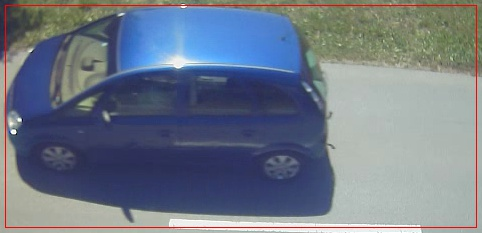
\includegraphics[width=0.49\textwidth]{Testversuche/GrabCut1.jpg}}
  \subfigure[Ergebnis des Algorithmus]{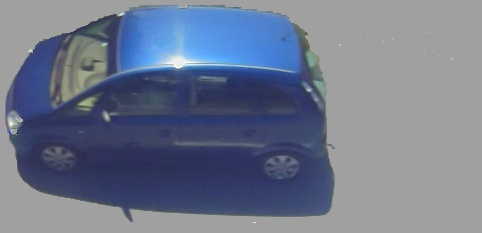
\includegraphics[width=0.49\textwidth]{Testversuche/GrabCut2.jpg}}
  \caption{Beispiel GrabCut}
  \label{bGrabCut}
\end{figure}

Auf dem linken Bild sind das Originalbild und der definierte Rahmen zu sehen, auf dem rechte Bild das Ergebnis dazu. Dem Ergebnis wurde ein grauer Hintergrund hinzugefügt, jedoch kann diese Farbe frei gewählt werden. Je nach Bild, welches verwendet wird, kann GrabCut schlechte bis hervorragende Resultate liefern. Dabei kommt es vor allem darauf an, wie starke Farbveränderungen im Hintergrund vorhanden sind. Bei diesem Algorithmus handelt es sich um eine komplexe Methode, welche selbst auf dem Computer einige Sekunden an Verarbeitungszeit benötigt. \cite{GrabCut}

\subsubsection{Schattenentfernung}